\mychapter{Detecção e diagnóstico de falhas}
\label{cap:detec_diag}

Com a demanda cada vez mais crescente com relação a eficiência, a qualidade dos
produtos e a integração dos processos no setor industrial, aliada aos altos
custos envolvidos e as mais diversas necessidades de segurança, torna-se
evidente a importância dos sistemas de supervisão e dos sistemas de Detecção e
Diagnóstico de Falhas (DDF) \cite{isermann:2006}.

Atualmente, devido ao nível de complexidade envolvido em um processo industrial,
os sistemas de supervisão e proteção exigem as mais avançadas técnicas
oferecidas pela engenharia moderna e, ainda assim, demandam um esforço contínuo
por parte dos pesquisadores e engenheiros para que sejam desenvolvidas novas
tecnologias que venham a suprir suas necessidades \cite{silva:2008}.

Considerando tais aspectos, este capítulo mostrará os conceitos relacionados ao
desenvolvimento de um sistema de DDF que fará uso de RNAs. Inicialmente, serão
mostrados os principais conceitos e terminologias utilizadas na área, destacando
alguns dos métodos para a realização de DDF.

% ------------------------------------------------------------------------------
\section{Conceitos e terminologias}\label{sec:propriedades}
Segundo \citeasnoun{kaanich:2002}, os sistemas computacionais podem ser
caracterizados por cinco propriedades fundamentais: funcionalidade, usabilidade,
desempenho, custo e {\it dependabilidade}. Para \citeasnoun{laprie:1992}, o
termo {\it dependabilidade}, que nada mais é do que a tradução literal do termo
inglês {\it dependability}, está relacionado com a capacidade de um sistema
prestar um serviço que possa ser, justificadamente, confiável. O serviço
prestado se refere ao comportamento do sistema percebido por seus usuários, os
quais também serão sistemas (máquinas físicas ou seres humanos), que interagem
com o anterior.

De acordo com \citeasnoun{laprie:1994}, dependendo das aplicações envolvidas, o
termo dependabilidade pode ainda ser visto a partir de suas diferentes, mas,
complementares, propriedades:

\begin{itemize}
    \item {\bf Disponibilidade:} Prontidão para o uso;
    \item {\bf Confiabilidade:} Continuidade do serviço;
    \item \textbf{Proteção (\textit{safety}):} Não ocorrência de consequências
          catastróficas para o meio;
    \item {\bf Confidencialidade:} Não ocorrência da divulgação não-autorizada
          da informação;
    \item {\bf Integridade:} Não ocorrência de alterações indevidas da
          informação;
    \item {\bf Manutenção:} Aptidão para sofrer reparos e evolução.
\end{itemize}

A associação da integridade com a disponibilidade e a confidencialidade leva à
\textbf{Segurança (\textit{security})}.

Apesar do termo dependabilidade ser utilizado na maioria das vezes dessa forma,
o dicionário Michaelis, traduz tal termo como {\it confiabilidade} ou {\it
garantia de funcionamento}. Assim sendo, daqui para frente, a palavra {\it
confiável}, ou suas variações linguísticas, também será utilizada para se
referir ao termo {\it dependable}. Se for necessário fazer referência a
propriedade da confiabilidade de um sistema, tal intenção será claramente
especificada pelo texto.

% ------------------------------------------------------------------------------
\section{Sistemática da dependabilidade}
\citeasnoun{avizienis:2000} e \citeasnoun{kaanich:2002} mostram que para se
desenvolver um Sistema Computacional Confiável (SCC, do inglês {\it Dependable
Computing System} -- DCS), faz-se uso de diferentes técnicas, tais como as
técnicas de: {\bf prevenção}, {\bf tolerância}, {\bf supressão} e {\bf previsão}
de falhas.

O estudo sobre a {\it prevenção} de falhas envolve a seleção de metologias de
projeto e de tecnologias adequadas para a escolha e a aplicação dos componentes
no sistema, ou seja, busca não introduzir ou evitar que as falhas aconteçam. A
{\it tolerância} a falhas está mais relacionada com a continuidade da prestação
do serviço quando uma falha vier a ocorrer. Algumas das aplicações mais
conhecidas são: mascaramento de falhas, redundância de dispositivos/sistemas e a
detecção/recuperação de falhas. A {\it supressão} das falhas procura minimizar
as consequências relativas à presença de uma falha através de mecanismos de
verificação, diagnóstico e correção. A {\it previsão} de falhas está relacionada
com a estimativa que pode ser feita sobre a presença, a criação e a consequência
que as falhas venham a causar no sistema. Para isso, tal técnica faz uso de
critérios avaliativos, técnicas de injeção de falhas e testes de resistência.

Além dessas técnicas, é válido também fazer referência aos termos {\bf avaria}
({\it failure}), {\bf erro} ({\it error}) e {\bf falha} ({\it fault}),
conceitualmente abordados de diferentes maneiras por vários autores. Os
conceitos relativos a essa nomenclatura serão melhor explicados na seção
\ref{sec:avaria_erro_falha}.

\begin{comment}
\begin{itemize}
    \item {\bf Técnicas de prevenção:} Como prevenir a ocorrência ou a introdução de
          falhas;
    \item {\bf Técnicas de tolerância:} Como oferecer um serviço ``correto'' na
          presença de falhas;
    \item {\bf Técnicas de supressão:} Como reduzir o número ou atenuar a
          gravidade das falhas;
    \item {\bf Técnicas de previsão:} Como estimar o número atual, a incidência
          futura e as consequências das prováveis falhas.
\end{itemize}
\end{comment}

A partir dessas informações, \citeasnoun{avizienis:2000} classifica os termos
acima relacionados em três grupos, denominados atributos (propriedades), ameaças
e meios pelos quais a dependabilidade é atingida, conforme pode ser observado
na Fig. \ref{fig:div_avizienis}.

\begin{figure}[htb]
\centering
\footnotesize
\[
\text{Dependabilidade}
\left\{
\begin{array}{l}
\text{Atributos}
    \left\{
    \begin{array}{l}
        \text{Disponibilidade}\\
        \text{Confiabilidade}\\
        \text{Proteção}\\
        \text{Confidencialidade}\\
        \text{Integridade}\\
        \text{Manutenção}\\
        \text{Segurança}
    \end{array}
    \right.
\\
\\
\text{Ameaças}
    \left\{
    \begin{array}{l}
        \text{Avaria ({\it failure})}\\
        \text{Erro ({\it error})}\\
        \text{Falha ({\it fault})}
    \end{array}
    \right.
\\
\\
\text{Meios}
    \left\{
    \begin{array}{l}
        \text{Prevenção}\\
        \text{Tolerância}\\
        \text{Supressão}\\
        \text{Previsão}
    \end{array}
    \right.
\end{array}
\right.
\]
\caption{Classificação sistemática da dependabilidade.}
\label{fig:div_avizienis}
\end{figure}

O primeiro grupo, cujos elementos foram brevemente explicados na seção
\ref{sec:propriedades}, permite expressar as propriedades esperadas e analisar a
qualidade de um sistema confiável. Já o segundo grupo traz os termos utilizados
para expressar características indesejadas -- mas, em princípio, não inesperadas
-- que causam ou fazem com que um sistema passe a ser não-confiável. Por fim, o
terceiro grupo exibe os meios ou as técnicas pelas quais torna-se possível
oferecer um serviço confiável.

De posse dessas informações e sabendo que muitas vezes os autores utilizam
traduções diferentes para {\it failure}, {\it error} e {\it fault}, a seção
seguinte tentará esclarecer o significado de cada um desses termos.

% ------------------------------------------------------------------------------
\section{Avarias, erros e falhas}\label{sec:avaria_erro_falha}
Em um processo real, todos os recursos utilizados, sejam físicos ou
implementados em {\it software}, estão sujeitos a interrupções ou a
comprometimentos operacionais.

Em sistemas críticos, tais como as aeronaves ou as usinas nucleares, essas
situações fazem com que pequenos ``deslizes operacionais'' venham a trazer
grandes e indesejáveis consequências. Como exemplo dessas consequências, pode-se
destacar o acidente do {\it Airbus 320} da TAM em 2007, que não conseguiu parar
ao aterrissar no aeroporto de Congonhas, São Paulo, no qual morreram 199 pessoas
(12 em solo e 187 no avião) e o desastre da usina nuclear de Chernobil, que
liberou cerca de 400 vezes mais contaminação do que a bomba nuclear que foi
lançada em Hiroshima.

Esses exemplos fazem com que se reflita sobre como os sistemas de controle podem
evoluir para evitar que catástrofes ainda maiores venham a ocorrer. Ou seja,
como as propriedades de um sistema de controle confiável poderão ser mantidas
mesmo na presença de avarias, erros e falhas no processo.

Segundo \citeasnoun{nelio:2002}, apesar do termo falha ser utilizado, em muitos
dos casos, como um termo vago, abrangendo também o significado de avarias e
erros, existem certas diferenças conceituais que devem ser observadas.

O termo {\bf avaria} ({\it failure}) deve ser utilizado para indicar que houve
um desvio do comportamento no sistema, o que o torna incapaz de fornecer o
serviço para o qual foi designado. Um {\bf erro} ({\it error}), entretanto, está
relacionado com estado do sistema e pode levar a uma avaria. De maneira
resumida, se há um erro no estado do sistema, então existe uma sequência de
ações que podem ser executadas e que levarão as avarias, a não ser que medidas
corretivas venham a ser tomadas. Por fim, mas não menos importante, o termo {\bf
falha} ({\it fault}) é a causa de um erro e está associado à noção de defeitos.
Normalmente, diz-se que o termo falha pode ser definido como sendo um defeito
que possui o potencial de gerar erros \cite{nelio:2002,weber:2002}.

Conforme dito anteriormente, alguns autores costumam traduzir os termos {\it
failure}, {\it error} e {\it fault} de maneira diferente. O termo {\it failure},
por exemplo, também é traduzido como falha e o termo {\it fault} como falta.
Entretanto, como é mais comum se referir a sistemas de controle tolerante a
``falhas'' ao invés de sistemas de controle tolerantes a ``faltas'', preferiu-se
aqui traduzir o termo {\it failure} como avaria e o termo {\it fault} como
falha, até mesmo porque as avarias ({\it failures}) não podem ser toleradas.

\begin{comment}
Por esse motivo, ao longo do texto, quando for necessário se referir ao termo
{\it failure}, será utilizada a palavra avaria. Já o termo falha será utilizado
de maneira mais abrangente, envolvendo os conceitos de erro e de falha
explicados anteriormente.
\end{comment}

Tendo conhecido o significado de cada um desses termos, pode-se mostrar que
existe uma certa relação entre eles. Considerando que os sistemas reais são
normalmente compostos por subsistemas, é comum se observar que uma falha leva a
um erro, que por sua vez pode levar a uma avaria, podendo vir a gerar novas
falhas e dar início a uma reação em cadeia, tal como mostra a Fig.
\ref{fig:reacao_cadeia}. Contudo, nem sempre uma falha conduz a um erro, assim
como nem sempre um erro conduz a uma avaria, mas todos os erros resultam de
falhas e todas as avarias resultam de erros.

\begin{figure}[htb]
\centering
\[
\ldots
\quad\Longrightarrow\quad
\text{Falha} 
\quad\longrightarrow\quad
\text{Erro}
\quad\longrightarrow\quad
\text{Avaria}
\quad\Longrightarrow\quad
\text{Falha}
\quad\longrightarrow\quad
\ldots
\]
    \caption{Reação em cadeia das falhas, erros e avarias.}
    \label{fig:reacao_cadeia}
\end{figure}

Uma outra maneira de visualizar as relações existentes entre cada um desses
termos pode ser observada na Fig. \ref{fig:mapa_conceitos}.

\begin{figure}[htb]
\centering
    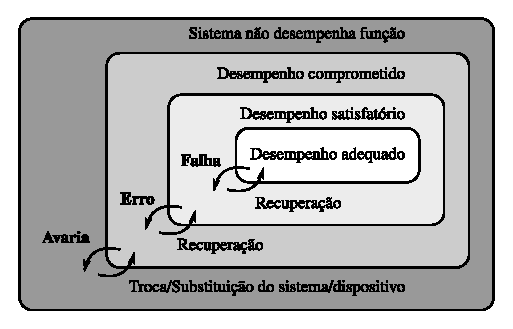
\includegraphics[width=0.5\textwidth]{imgs/detec_diag/eps/mapa_conceitos}
    \caption{Mapa de conceitos relacionados a avarias, erros e falhas em um
             sistema.}
    \label{fig:mapa_conceitos}
\end{figure}

\citeasnoun{weber:2002} afirma que as falhas são inevitáveis, uma vez que os
componentes físicos do sistema envelhecem e estão sempre sujeitos as
interferências externas, ambientais ou humanas. Mostra ainda que os {\it
softwares}, assim como os sistemas físicos, também são vítimas de falhas, pois
estão a mercê da alta complexidade dos processos e da fragilidade humana em
trabalhar com grande volume de detalhes de especificação e operação.

% ------------------------------------------------------------------------------
\subsection{Tipos de falhas}

\begin{comment}
\citeasnoun{laprie:1994} mostra que existem cinco classes elementares para as
falhas, conforme Fig. \ref{fig:class_laprie}.

\begin{figure}[htb]
\centering
\footnotesize
\[
\text{Falha}
\left\{
\begin{array}{l}
\text{Causas fenomenológicas}
    \left\{
    \begin{array}{l}
        \text{Falhas físicas}\\
        \text{Falhas humanas}
    \end{array}
    \right.
\\
\\
\text{Natureza}
    \left\{
    \begin{array}{l}
        \text{Falhas acidentais}\\
        \text{Falhas intencionais, não-maliciosas}\\
        \text{Falhas intencionais, maliciosas}
    \end{array}
    \right.
\\
\\
\text{Criação/Ocorrência}
    \left\{
    \begin{array}{l}
        \text{Falhas de desenvolvimento}\\
        \text{Falhas operacionais}
    \end{array}
    \right.
\\
\\
\text{Limitações do sistema}
    \left\{
    \begin{array}{l}
        \text{Falhas internas}\\
        \text{Falhas externas}
    \end{array}
    \right.
\\
\\
\text{Persistência}
    \left\{
    \begin{array}{l}
        \text{Falhas permanentes}\\
        \text{Falhas temporárias}
    \end{array}
    \right.
\end{array}
\right.
\]
    \caption{As cinco classes elementares das falhas.}
    \label{fig:class_laprie}
\end{figure}

\end{comment}

De acordo com \citeasnoun{silva:2008}, as falhas em um processo industrial podem
ser classificadas em relação a vários aspectos. Em se tratando da classificação
quanto ao tempo, as falhas podem ser abruptas, incipientes ou intermitentes, tal
como mostra a Fig. \ref{fig:tipos_falha}.

\begin{figure}[H]
\centering
    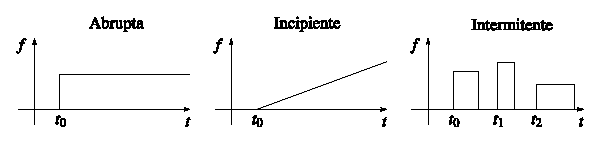
\includegraphics[width=0.75\textwidth]{imgs/detec_diag/eps/tipos_falha}
    \caption{Características temporais das falhas quanto a sua persistência.}
    \label{fig:tipos_falha}
\end{figure}

\begin{comment}
De acordo com essa classificação, percebe-se que não existirá um sistema
que venha a falhar somente uma vez. Por mais que as falhas demorem a acontecer,
elas são inevitáveis.
\end{comment}

As {\it falhas abruptas} surgem repentinamente, podendo ser decorrentes de
imprevistos ou até mesmo de acidentes. Essas falhas mudam o comportamento do
processo rapidamente, exigindo contra-ações velozes e eficazes que possam
minimizar as consequências do ocorrido.

As {\it falhas incipientes} iniciam a partir de pequenos desvios comportamentais
do sistema, podendo ser mascaradas pelos controladores. Muitas vezes essas
falhas acabam passando despercebidas pelos operadores ou até mesmo pelos
sistemas de detecção e diagnóstico de falhas.

As {\it falhas intermitentes} são aquelas que ocorrem durante um certo período
de tempo e, em seguida, desaparecem, voltando a aparecer após um novo intervalo.
Podem ser causadas por alguma perturbação periódica ou por alguma situação que
se repita ciclicamente.

Com relação a localização das falhas, estas podem ocorrer nos sensores, nos
atuadores ou na estrutura do sistema \cite{silva:2008}. As {\it falhas nos
sensores} são observadas através de variações específicas nas medições, as quais
podem ser descaracterizadas como variações válidas do sistema. As {\it falhas
nos atuadores} podem ser vistas como qualquer mau funcionamento do equipamento
que atua no sistema. As {\it falhas na estrutura}, ou {\it falhas estruturais},
ocorrem quando alguma alteração do sistema muda, de alguma forma, a relação
original de entrada e saída do processo ou quando ocorre algum problema com
algum dos dispositivos, desde que não sejam sensores ou atuadores, como por
exemplo, os transmissores de sinal. Considerando então um processo genérico,
pode-se citar como exemplos de falhas aquelas exibidas pela Tab.
\ref{tab:falhas}.

\begin{table}[htb]
\small
\centering
\caption{Exemplos de falhas para um processo genérico.}
\label{tab:falhas}
\vspace{0.25cm}
\begin{tabular}{|c|c|c|}
\hline
{\bf Sensores} & {\bf Atuadores} & {\bf Estrutura}\\
\hline
\hline
Erro de leitura & Erro de escrita & Erro de transmissão\\
\hline
Descalibramento & Erro de leitura & Perda de comunicação\\
\hline
Sensibilidade a ruído & Sensibilidade a ruído & Sensibilidade a ruído
(transmissor)\\
\hline
Queima & Queima & Queima (transmissor)\\
\hline
- & Atraso de transporte & Atraso de propagação de sinais\\
\hline
\end{tabular}
\end{table}

Maiores detalhes sobre as propriedades e a classificação das falhas podem ser
encontradas em \citeasnoun{laprie:1992}, \citeasnoun{laprie:1994},
\citeasnoun{weber:2002} e \citeasnoun{isermann:2006}.

% ------------------------------------------------------------------------------
%\section{Os meios para se atingir a dependabilidade}
%\label{sec:tecnicas}

% ------------------------------------------------------------------------------
\section{Detecção e diagnóstico de falhas}
Considerando que os processos industrias estão se tornando cada vez mais integrados e
complexos, a ocorrência de falhas passa a ser mais um fator de complicação. As
falhas que antes poderiam ser detectadas facilmente por medições diretas de
determinada variável dependem agora de um conjunto de variáveis que atuam
simultaneamente no sistema. 

Além disso, se uma falha é detectada em um determinado ponto de um sistema, a
causa do problema pode estar próxima ou distante, dependendo do grau de
complexidade envolvido. Como exemplo, uma simples falha em uma aeronave pode
causar indicações de falha em diversos subsistemas de segurança
\cite{vach:2006}. Dessa maneira, processar as informações disponíveis pode vir a
contribuir de maneira significativa para o processo de detecção e diagnóstico de
falhas.

Com o intuito de garantir o sucesso das operações planejadas e reconhecer as
anomalias comportamentais dos processos, muitos sistemas de supervisão e
monitoramento estão sendo desenvolvidos. Para \citeasnoun{chiang:2001},
dentre diversas outras funções, esses sistemas podem auxiliar nas atividades de
detectar, diagnosticar e suprimir falhas, garantindo que as operações do
processo satisfaçam as especificações de desempenho.

De maneira complementar, destaca-se que a informação a ser disponibilizada por
um sistema de monitoramento não deve, tão somente, informar ao operador do
sistema sobre o que está acontecendo, mas auxiliá-lo a tomar medidas corretivas
com o intuito de sanar o problema. Como resultado disso, o tempo em que o
sistema estará inoperante será reduzido, a proteção do sistema aumentará e os
custos relacionados diminuirão.

Para \citeasnoun{chiang:2001}, existem quatro fases envolvidas no monitoramento
dos processos: {\bf detecção}, {\bf isolamento}, {\bf diagnóstico} e {\bf
recuperação} de falhas, conforme mostrado pela Fig.
\ref{fig:fases_monitoramento}.

\begin{figure}[htb]
\centering
    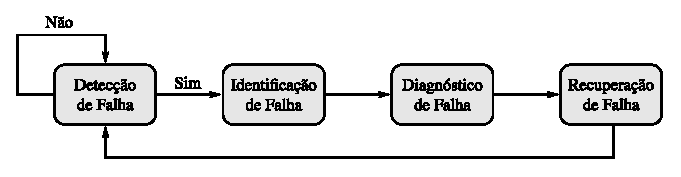
\includegraphics[width=0.7\textwidth]
                    {imgs/detec_diag/eps/fases_monitoramento}
    \caption{Fases envolvidas no monitoramento de processos.}
    \label{fig:fases_monitoramento}
\end{figure}

A {\it detecção da falha} se resume a determinar se ocorreu ou não uma falha.
Quando realizada de maneira antecipada, a detecção de falhas pode fornecer
informações valiosas com relação aos problemas que estão por acontecer.  Assim,
através de ações apropriadas, pode-se evitar grandes perturbações no processo.

A {\it identificação da falha} tem por objetivo identificar as variáveis mais
importantes para que se realize um diagnóstico apropriado. Para isso, essa fase
procura concentrar as atenções do operador nos subsistemas mais pertinentes à
falha, de tal modo que o efeito desta possa ser eliminado de maneira mais
eficiente.

A fase de {\it diagnóstico da falha} determina que falha ocorreu. De acordo com
\citeasnoun{isermann:2004}, essa fase deverá indicar o maior número de detalhes
possíveis a respeito da falha, tais como a intensidade, a localização e o
momento em que a falha foi detectada. Essa fase é considerada essencial para uma
contra-ação ou eliminação da falha.

Por fim, a fase de {\it recuperação da falha}, também conhecida como fase de
{\it intervenção}, tem por objetivo remover o efeito da falha para com o
sistema, dando início a um novo ciclo de detecção e diagnóstico.

Apesar de estarem explicitamente colocados como uma sequência de ações, nem
sempre todas as fases são estritamente necessárias \cite{chiang:2001}. Os
sistemas automatizados fazem com que a mudança de uma fase para outra seja
transparente para operador, exibindo apenas as informações cruciais para que se
possa tomar as medidas cabíveis.

\citeasnoun{venkatasu:2003a} mostram que a automatização das formas de detecção
e diagnóstico é o primeiro passo a ser tomado para a elaboração de um sistema de
gestão de eventos anormais. Afirmam também que ao longo de vários anos muitas
soluções vem sendo desenvolvidas e que um grande número de técnicas já foram
utilizadas. Para isso, citam como exemplos as técnicas que utilizam árvores de
falhas, digrafos, abordagens analíticas, sistemas especialistas e RNAs.

\fussy
Do ponto de vista de modelagem, existem métodos que exigem grande precisão com
relação ao modelo de processo, outros que exigem modelos semi-quantitativos ou
ainda modelos qualitativos. Por outro lado, existem métodos que não necessitam
de nenhuma informação do modelo, os quais utilizam somente as informações de
histórico do processo \cite{venkatasu:2003a}.
\sloppy

Conforme mostrado no Capítulo \ref{cap:introducao}, a classificação dos métodos
de DDF pode variar de autor para autor
\cite{venkatasu:2003a,angeli:2004,zhang:2008,isermann:2006}. A abordagem aqui
escolhida irá considerar a classificação adotada em \citeasnoun{isermann:2006},
até então considerada mais intuitiva.

% ------------------------------------------------------------------------------
\section{Métodos de detecção}
Nas seções seguintes será feita uma breve análise dos métodos de detecção de
falhas abordados em \citeasnoun{isermann:2006}. Vale salientar que existem na
literatura vários outros métodos de detecção de falhas. Deseja-se aqui apenas
trazer alguns exemplos.

% ------------------------------------------------------------------------------
\subsection{Detecção de falhas com verificação de limites}
Considerado como um dos métodos mais simples e intuitivos, a detecção de falhas
com verificação de limites baseia-se na medição direta de uma determinada
variável e a comparação de seu valor absoluto ou de sua tendência com um
limítrofe previamente especificado.

A verificação de valores absolutos baseia-se na utilização de dois limiares ou
limítrofes fixos, denominados $Y_{min}$ e $Y_{max}$. O funcionamento normal do
sistema consiste em verificar se a variável $Y$ está ou não contida no
intervalo:

\begin{equation}
Y_{min} < Y < Y_{max}
\end{equation}

Essa abordagem considera que o processo está funcionando normalmente quando a
variável monitorada encontra-se dentro de uma zona de tolerância. Quando a
variável monitorada excede um dos limiares estabelecidos, deduz-se que haverá
uma falha em algum ponto do processo. Por mais simples que pareça, este método é
aplicado na maioria dos sistemas de automação

A outra abordagem utiliza a tendência da variável medida para detectar as
falhas. Como exemplo, um dos métodos mais conhecidos faz uso da primeira
derivada da variável ($\dot{Y} = dY(t)/dt$) e testa se a variação observada está
ou não dentro de uma faixa previamente estabelecida:

\begin{equation}
\dot{Y}_{min} < \dot{Y} < \dot{Y}_{max}
\end{equation}

Exemplos dessas duas abordagens podem ser observados na Fig.
\ref{fig:detec_ver_lim}.

\begin{figure}[htb]
\centering
    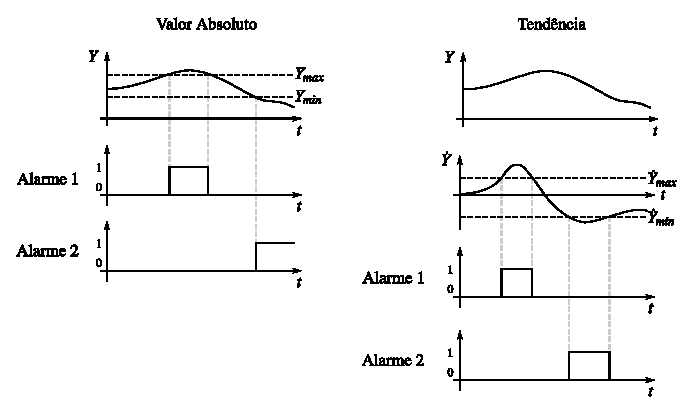
\includegraphics[width=0.85\textwidth]{imgs/detec_diag/eps/detec_ver_lim}
    \caption{Exemplo de detecção com verificação de limites.}
    \label{fig:detec_ver_lim}
\end{figure}

% ------------------------------------------------------------------------------
\subsection{Detecção de falhas com modelos de sinais}
Diversos sinais medidos em um processo apresentam oscilações de natureza
harmônica ou estocástica. Se as mudanças nesse sinal estiverem relacionadas com
as falhas nos sensores, atuadores ou estruturais, pode-se detectar essas falhas
através do uso de modelos de sinais.

Considera-se, portanto, que as características do sinal medido, tais como
amplitude, fase, espectro de frequências, dentre outras, são calculadas a partir
de modelos matemáticos do sinal e comparadas com as características observadas
durante o funcionamento normal. As diferenças comportamentais geradas pela
comparação, denominadas de {\it sintomas analíticos}, são utilizadas para
realizar a detecção das falhas.

Na Fig. \ref{fig:detec_mod_sin} é exibido um diagrama esquemático que resume os
princípios da detecção de falhas com modelos de sinais.

\begin{figure}[htb]
\centering
    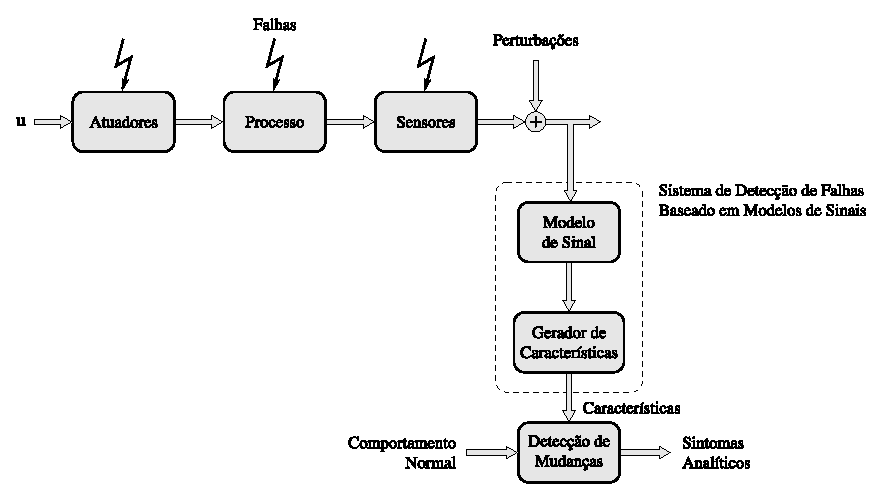
\includegraphics[width=0.95\textwidth]{imgs/detec_diag/eps/detec_mod_sin}
    \caption{Diagrama esquemático da detecção de falhas com modelos de sinais.}
    \label{fig:detec_mod_sin}
\end{figure}

% ------------------------------------------------------------------------------
\subsection{Detecção de falhas com equações de paridade}
Uma das formas de se detectar falhas de maneira direta em um processo baseia-se
na comparação do comportamento real com o comportamento nominal. A diferença
entre os sinais de saída do processo real e os sinais de saída do modelo
matemático que descreve sua dinâmica geram os {\it resíduos} utilizados para
detecção da falha. De acordo com \citeasnoun{silva:2008}, os resíduos são a base
de várias abordagens de sistemas de Detecção e Isolamento de Falhas (DIF). A
Fig. \ref{fig:residuos} e a Eq. \ref{eq:residuos} mostram como os resíduos são
obtidos para um sistema de múltiplas entradas e múltiplas saídas ({\it Multiple
Input and Multiple Output} -- MIMO).

\Glossary{MIMO}{\it Multiple Input and Multiple Output}

\begin{figure}[htb]
\centering
    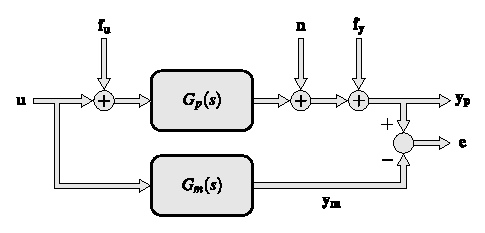
\includegraphics[width=0.6\textwidth]{imgs/detec_diag/eps/residuos}
    \caption{Obtenção dos resíduos para um sistema MIMO.}
    \label{fig:residuos}
\end{figure}

\begin{eqnarray}\label{eq:residuos}
e(s) & = & y_p(s) - y_m(s) = y_p(s) - G_m(s)u(s)\nonumber\\
& = & G_p(s)\left[u(s) + f_u(s)\right] + n(s) + f_y(s) - G_m(s)u(s)\nonumber\\
& = & \left[G_p(s) - G_m(s)\right]u(s) + G_p(s)f_u(s) + n(s) + f_y(s)\nonumber\\
& = & \Delta G_m(s) u(s) + G_p(s)f_u(s) + n(s) + f_y(s)
\end{eqnarray}

Nessa equação, $f_u$ corresponde às falhas aditivas na entrada, $f_y$ às falhas
aditivas na saída, $n$ aos ruídos, $y_p$ à saída do processo, $y_m$ à saída do
modelo, $G_p$ à função de transferência do processo, $G_m$ à função de
transferência do modelo, $u$ às entradas e $e$ aos resíduos.

\Glossary{DIF}{Detecção e Isolamento de Falhas}

Apesar da capacidade em indicar anormalidades no processo através das
discrepâncias, essa abordagem possui a desvantagem de ser necessário se ter o
conhecimento prévio das equações que regem a dinâmica do processo. Devido a
dificuldade existente em se utilizar um modelo fenomenológico preciso, que leve
em consideração, inclusive, os ruídos naturalmente presentes no processo, esse
método não é muito utilizado.

% ------------------------------------------------------------------------------
\subsection{Detecção de falhas com métodos de identificação}
Os modelos matemáticos de processos descrevem uma relação entre os sinais de
entrada $u(t)$ e os sinais de saída $y(t)$. Em muitos dos casos não se conhece o
processo por completo, o que inviabiliza a elaboração de um modelo preciso que
leve em consideração os desvios comportamentais. Dessa forma, os métodos de
identificação de processos precisam ser frequentemente aplicados antes da
utilização de qualquer técnica de detecção de falhas.

Conforme mostra a Fig. \ref{fig:metodos_identificacao}, existem diversos métodos
de identificação de processos dinâmicos. A opção pela utilização de cada um
deles varia de acordo com a aplicação.

\begin{figure}[htb]
\centering
    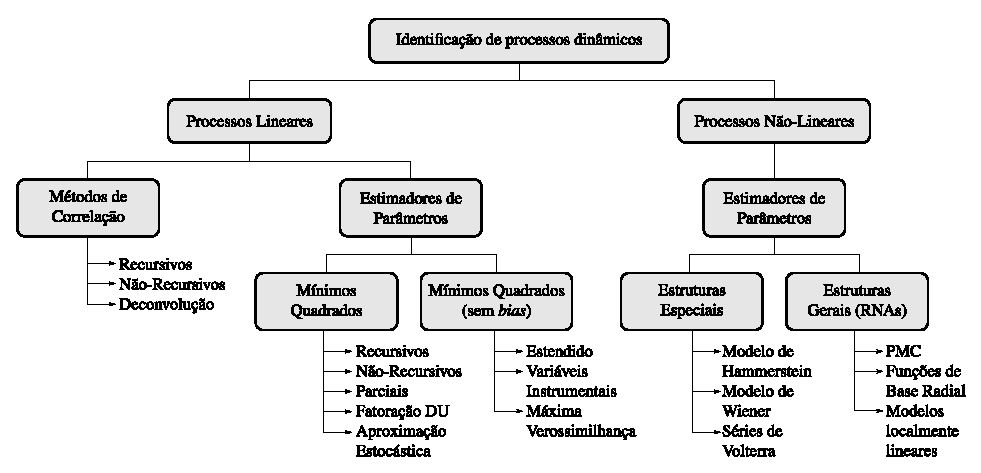
\includegraphics[width=\textwidth]{imgs/detec_diag/eps/metodos_identificacao}
    \caption{Árvore de métodos de identificação de processos dinâmicos.}
    \label{fig:metodos_identificacao}
\end{figure}

% ------------------------------------------------------------------------------
\subsection{Detecção de falhas com observadores e estimadores de estado}
Considerando que os observadores de estado utilizam o erro de saída, dado pela
diferença entre a medição da variável no processo e o modelo ajustável, pode-se
dizer que eles são bons candidatos a sistemas de detecção baseados em modelos.
Assume-se que, assim como no caso das abordagem que utiliza equações de
paridade, a estrutura e os parâmetros do modelo precisam ser conhecidos. Dessa
forma, os observadores de estado poderão ajustar as variáveis do modelo de
acordo com as condições iniciais e com a evolução do processo, considerando os
sinais medidos das variáveis de entrada e saída.

Um tipo de abordagem proposta para sistemas MIMO, leva em consideração um
conjunto de observadores de estado tal como mostra a Fig.
\ref{fig:conj_obs_est}. De acordo com \citeasnoun{isermann:2006}, este esquema
pode ser utilizado para detectar falhas aditivas em sensores. Outras abordagens
fazem uso do Filtro de Kalman (estimador de estados) e de observadores de saída. 

\begin{figure}[htb]
\centering
    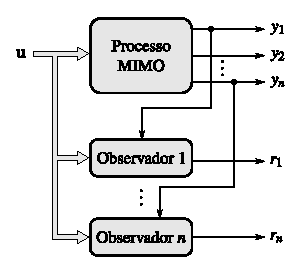
\includegraphics[width=0.345\textwidth]{imgs/detec_diag/eps/conj_obs_est}
    \caption{Detecção de falhas através de um conjunto de observadores de
             estado.}
    \label{fig:conj_obs_est}
\end{figure}
 
% ------------------------------------------------------------------------------
\section{Métodos de diagnóstico}
Para \citeasnoun{silva:2008} e \citeasnoun{isermann:2006} a tarefa de
diagnosticar uma falha consiste em determinar que uma falha ocorreu, indicando o
maior número de detalhes possíveis, tais como o momento de detecção, o tipo, a
localização e a intensidade da falha. Este procedimento de diagnóstico baseia-se
nos sintomas analíticos e nos conhecimentos heurísticos do processo.

A Fig. \ref{fig:diagnostico} sintetiza os passos necessários para o diagnóstico
de falhas, tanto para variáveis medidas de maneira automática, quanto para
variáveis observadas pelos operadores do processo. Em ambos os casos, a extração
de características relativas as alterações comportamentais sobre o processo são
necessárias. Os sintomas analíticos e heurísticos devem ser representados de
maneira unificada a fim de se realizar o diagnóstico de maneira adequada.

\begin{figure}[htb]
\centering
    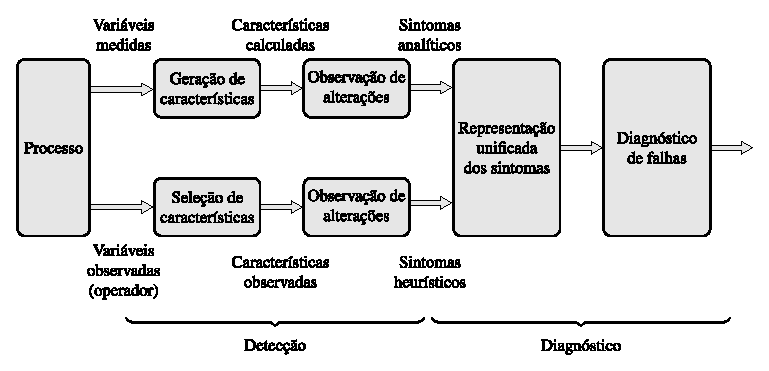
\includegraphics[width=0.9\textwidth]{imgs/detec_diag/eps/diagnostico}
    \caption{Sequências de passos que levam ao diagnóstico de falhas.}
    \label{fig:diagnostico}
\end{figure}

Vale observar que as {\it características} são os valores obtidos a partir dos
sinais ou de modelos de sinais do processo, os quais descrevem o seu estado
atual. Já os {\it sintomas} são as possíveis alterações das características com
relação a seus valores normais.

As relações entre uma falha e seus sintomas seguem normalmente as relações
físicas de causa e efeito. De maneira geral, pode-se dizer que uma falha produz
``eventos'' que por sua vez geram sintomas, conforme observado na Fig.
\ref{fig:falha_sintoma}. O diagnóstico de falhas normalmente é realizado de
maneira inversa, pois o sistema deve indicar as falhas a partir dos sintomas
observados.

\begin{figure}[htb]
\centering
    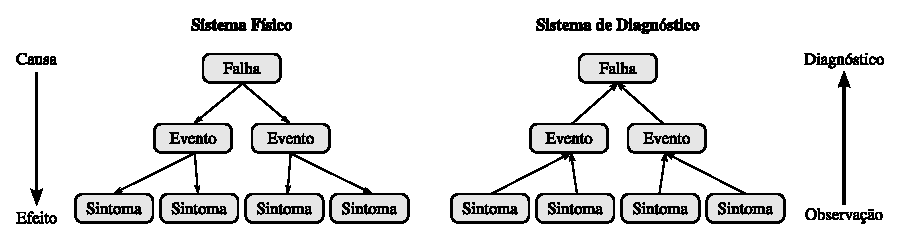
\includegraphics[width=\textwidth]{imgs/detec_diag/eps/falha_sintoma}
    \caption{Relações de falhas e sintomas.}
    \label{fig:falha_sintoma}
\end{figure}

\begin{comment}
% ------------------------------------------------------------------------------
\subsection{Diagnóstico de falhas com métodos de classificação}

% ------------------------------------------------------------------------------
\subsection{Diagnóstico de falhas com métodos de inferência}
\end{comment}

% ------------------------------------------------------------------------------
\section{Detecção e diagnóstico de falhas com RNAs}
Com a introdução das novas tecnologias de medição e o consequente aumento do
número de instrumentos nos processos industrias, o número de informações
disponíveis para um dado sistema tornou-se demasiadamente grande. Tal situação
acaba por aumentar ainda mais a complexidade de processamento, tendo em vista
que cada vez mais os procedimentos de DDF utilizam dados de histórico do
processo. Dentre os exemplos desses métodos que fazem uso de histórico do
processo estão aqueles são baseados em RNAs.

De acordo com a Fig. \ref{fig:metodos_identificacao}, as RNAs estão
classificadas como sendo estimadores de parâmetros de características gerais,
utilizadas para a identificação de sistemas dinâmicos baseados em modelos de
processos não-lineares. Já na Fig. \ref{fig:arvore_diagnostico}, as RNAs
aparecem como métodos de inferência que aproximam o raciocínio humano.

Unindo essas características com aquelas expostas no Cap. \ref{cap:rnas}, serão
utilizadas nesse trabalho duas estruturas compostas por redes neurais, com o
objetivo de identificar o processo de estudo de caso e realizar a detecção e o
diagnóstico de falhas a partir de seu histórico. As estruturas propostas serão
apresentadas no Cap. \ref{cap:sistema}, no momento em que forem mostrados
maiores detalhes sobre o processo em questão.
